\documentclass[12pt,a4paper]{article}

\renewcommand*\contentsname{Sadržaj}
\renewcommand{\figurename}{Slika}

\usepackage[margin=0.85in]{geometry}
\usepackage{graphicx}
\usepackage{float}
\usepackage{listings}
\usepackage{multirow}

% Default fixed font does not support bold face
\DeclareFixedFont{\ttb}{T1}{txtt}{bx}{n}{12} % for bold
\DeclareFixedFont{\ttm}{T1}{txtt}{m}{n}{12}  % for normal

% Custom colors
\usepackage{color}
\definecolor{deepblue}{rgb}{0,0,0.5}
\definecolor{deepred}{rgb}{0.6,0,0}
\definecolor{deepgreen}{rgb}{0,0.5,0}

% Python style for highlighting
\newcommand\pythonstyle{\lstset{
language=Python,
basicstyle=\ttm,
otherkeywords={self},             % Add keywords here
keywordstyle=\ttb\color{deepblue},
emph={MyClass,__init__},          % Custom highlighting
emphstyle=\ttb\color{deepred},    % Custom highlighting style
stringstyle=\color{deepgreen},
frame=tb,                         % Any extra options here
showstringspaces=false            % 
}}


% Python environment
\lstnewenvironment{python}[1][]
{
\pythonstyle
\lstset{#1}
}
{}

% Python for external files
\newcommand\pythonexternal[2][]{{
\pythonstyle
\lstinputlisting[#1]{#2}}}

% Python for inline
\newcommand\pythoninline[1]{{\pythonstyle\lstinline!#1!}}

% DODANO:
\renewcommand{\arraystretch}{1.5}
\begin{document}

\begin{titlepage}
	\centering
	{\scshape Univerzitet u Sarajevu \par}
	{\scshape Elektrotehnički Fakultet \par}
	\vspace{1cm}
	{\Large\scshape Prepoznavanje Oblika i Obrada Slike\par}
	\vspace{1.5cm}
	{\huge\bfseries Projektni Zadatak br. 2\par}
	\vspace{2cm}
	\Large Studenti: \par
	{\Large\itshape \textsc{Muftić} Belma, 1423/17260\par}
	{\Large\itshape \textsc{Lemeš} Lamija, 1474/17070\par}
	{\Large\itshape \textsc{Krupalija} Ehlimana, 1431/17461\par}
	\vfill
	Odgovorni asistent:\par
	MoE \textsc{Sumejja Porča}
	\vfill
	{\large December, 2018\par}
\end{titlepage}

\pagenumbering{gobble}

\tableofcontents

\newpage

\pagenumbering{arabic}
\setcounter{page}{1}

\section{Izbor modela za prepoznavanje}

Postoji šest najčešće korištenih klasifikacijskih modela (što je prikazano na Slici 1.):

\begin{enumerate}

\item SGD (\textit{Stohastic Gradient Descent}) klasifikacija;
\item \textit{Kernel Approximation} klasifikacija;
\item Linearna SVC (\textit{Support Vector Classification});
\item SVC (\textit{Support Vector Classification});
\item KNN (\textit{K-Nearest Neighbors}) klasifikacija;
\item \textit{Naive Bayes} klasifikacija.

\end{enumerate}

\begin{figure}[H]

\center
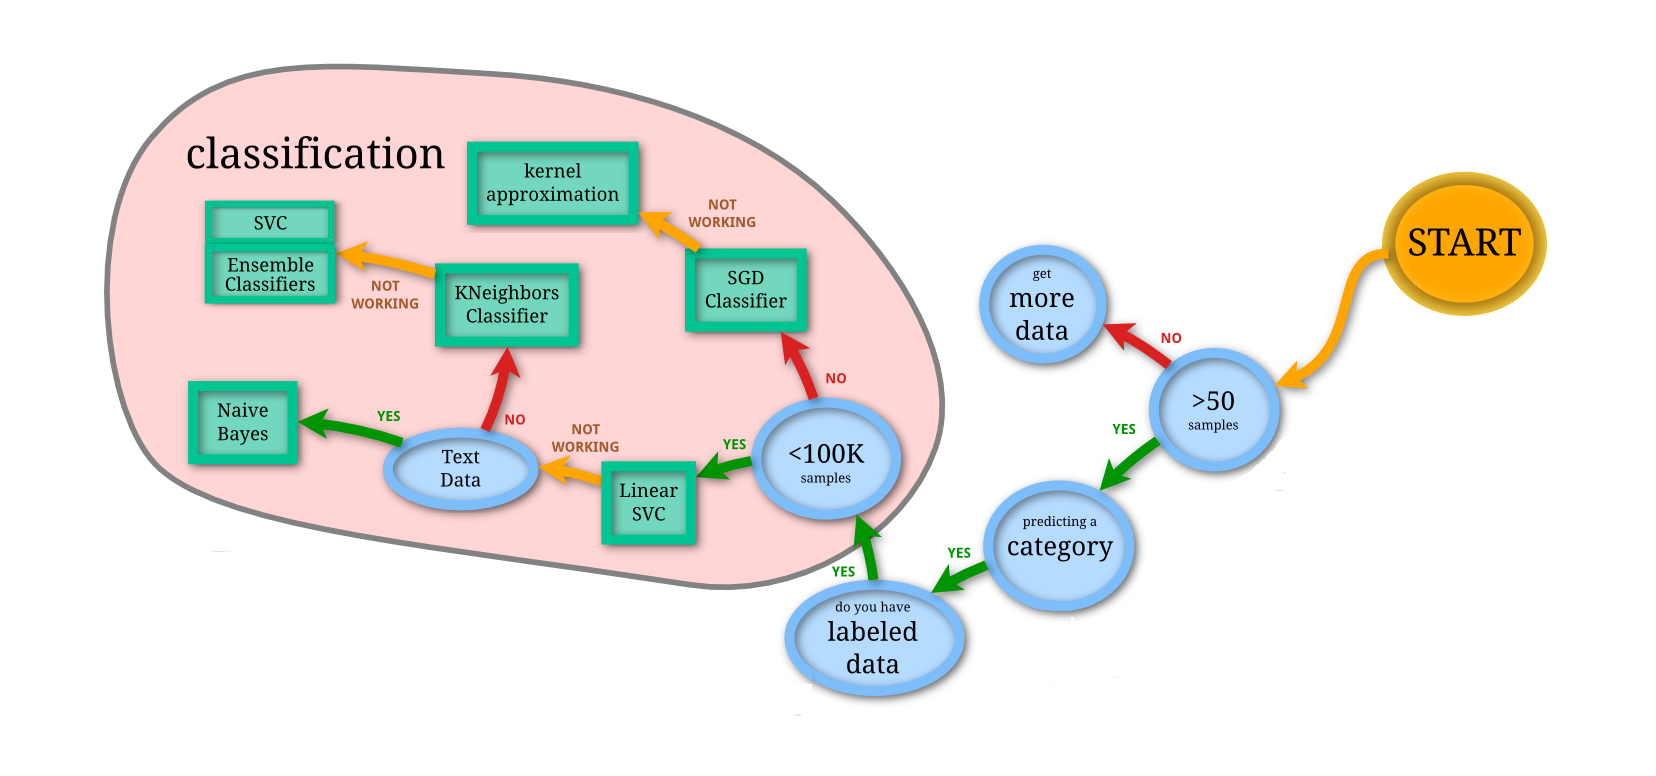
\includegraphics[scale=0.35]{slikaModeli.png}
\caption{Klasifikacijski modeli i vršenje njihovog odabira}
	
\end{figure}

Budući da \textit{dataset} ima manje od 100,000 slika, te postoje tekstualni podaci o različitim kategorijama i ROI, koristiti će se \textbf{\textit{Naive Bayes}} klasifikacijski model.

\newpage

\section{Izbor i kreiranje deskriptora}

Odabran je \textbf{\textit{HuMoments}} deskriptor, kako on opisuje oblik željenog objekta, a prepoznavanje ćelije se oslanja prvenstveno na njen oblik. U svrhu toga je kreirana skripta  \texttt{maskiranje.py} koja izloira samu ćeliju (dakle bez pozadine), jer se \textit{HuMoments} oslanja na analizu slika sa jednim kanalom.\\
~\\
Maskiranje je zasnovano na izdvajanju piksela koji spadaju u određeni rang vrijednosti, nakon čega se radi otvaranje da bi se uklonili ''zalutali'' pikseli, te se radi i dilatacija da bi se uključile i granice ćelije koje prethodno nisu bile u zadatom rasponu. Nakon maskiranja je pozvana funkcija \texttt{HuMoments} koja vraća niz brojeva koji opisuju oblik prethodno dobivene binarne slike. Nakon normalizacije niza, vrijednosti se zapisuju u CSV datoteku, te ako su u pitanju \textit{Train} slike, upisuje se i kojoj klasi slike pripadaju.\\
~\\
Navedene funkcionalnosti implementirane su na sljedeći način:\\

\pythonexternal{deskriptori.py}

\newpage

\section{Izbor metoda poboljšanja}

\subsection{Poboljšavanje kontrasta}

Od tri implementirane metode, najbolje rezultate pokazala je metoda \textbf{linearnog razvlačenja kontrasta}. Metoda aritmetičkih operacija previše je narušila strukturu slike, dok metoda \textit{gamma} korekcije nije izvršila dovoljnu modifikaciju kontrasta. Iz ovog razloga metoda linearnog razvlačenja kontrasta koristiti će se za poboljšavanje slika prije njihove dalje obrade.

\begin{figure}[H]

\center
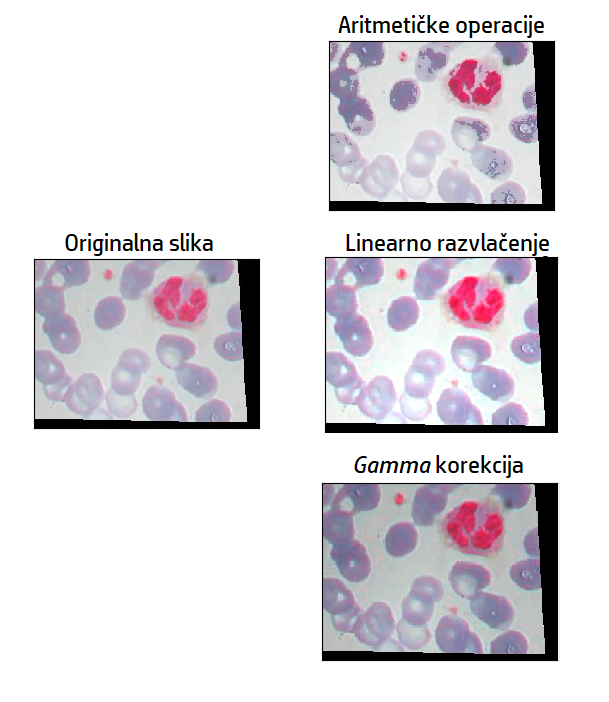
\includegraphics[scale=0.9]{slikaKontrast.png}
\caption{Rezultati korištenja različitih metoda za poboljšavanje kontrasta}
	
\end{figure}

\newpage

\subsection{Poboljšavanje osvjetljenja}

Od tri implementirane metode, najbolje rezultate pokazala je metoda \textbf{linearnih transformacija}. Metoda aritmetičkih operacija nije izvršila dovoljnu promjenu osvjetljenja, dok je metoda manipulacije HSV slikom izvršile preveliko povećanje osvjetljenja, te će se iz ovog razloga metoda linearnih transformacija koristiti za poboljšavanje slika prije njihove dalje obrade.

\begin{figure}[H]

\center
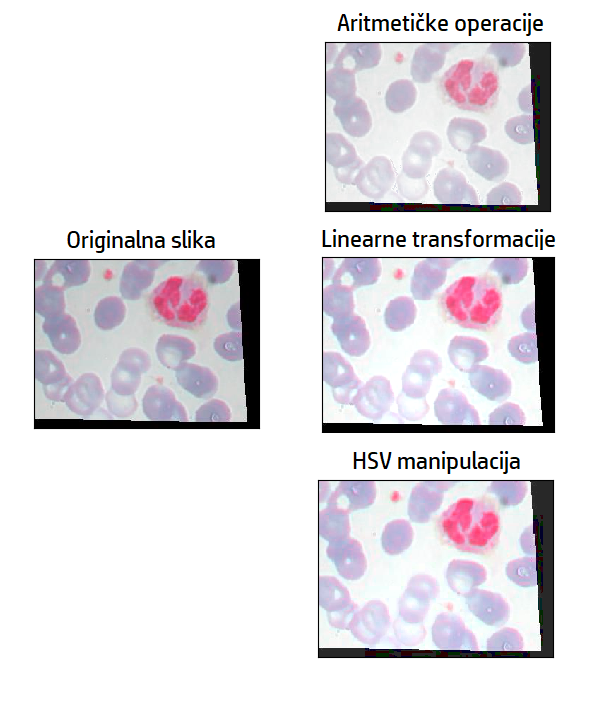
\includegraphics[scale=0.9]{slikaOsvjetljenje.png}
\caption{Rezultati korištenja različitih metoda za poboljšavanje osvjetljenja}
	
\end{figure}

\newpage

\subsection{Ujednačavanje histograma}

Od tri implementirane metode, najbolje rezultate pokazala je metoda \textbf{CLAHE}. Metoda raspodjele vjerovatnoća previše je degradirala strukturu slike (pri čemu su neke ćelije potpuno nestale sa slike, što je nedopustivo), dok je metoda \texttt{equalizeHist} degradirala strukturu slike u pogledu boje. Iz ovog razloga metoda CLAHE koristiti će se za poboljšavanje slika prije njihove dalje obrade.

\begin{figure}[H]

\center
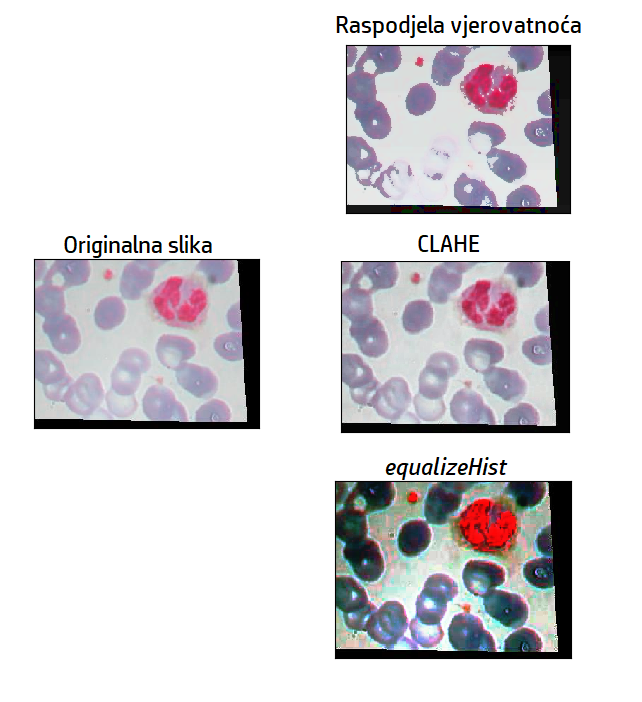
\includegraphics[scale=0.9]{slikaHistogram.png}
\caption{Rezultati korištenja različitih metoda za ujednačavanje histograma}
	
\end{figure}

\newpage

\section{Testiranje modela}

Kreirani deskriptori koriste se za treniranje i testiranje modela, pri čemu veoma važan aspekt predstavlja varijabla \texttt{confusionMatrix}, koja sadrži sve relevantne informacije o performansama modela. Na Slici 5. vidljivo je da je tačnost modela oko \textbf{76 \%}, te da najveću specifičnost pokazuje \textbf{klasa 1}, dok najveću senzitivnost pokazuje \textbf{klasa 2}. Najmanje vrijednosti specifičnosti i senzitivnosti ima \textbf{klasa 3}.

\begin{figure}[H]

\center
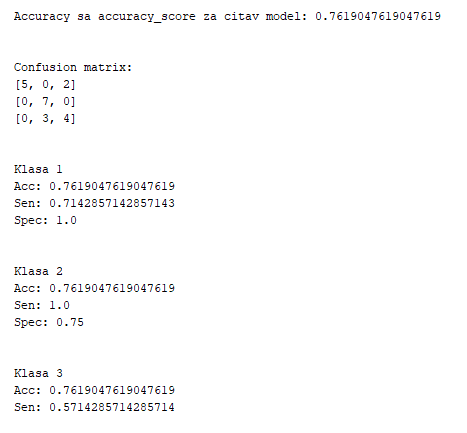
\includegraphics[scale=0.9]{slikaTest.png}
\caption{Rezultati pokretanja modela za prepoznavanje}
	
\end{figure}

\newpage

\section{Poboljšavanje performansi modela za prepoznavanje}

\subsection{Izmjena parametara modela}

Vrijednosti parametara tačnosti, specifičnosti i senzitivnosti za različite parametre modela prikazane su u sljedećim tabelama:

\begin{table}[H]
\centering
\begin{tabular}{|c|l|l|l|l|}
\hline
\textbf{\textit{Priors}}				& \textbf{\textit{Klasa}}   	& \textbf{\textit{Accuracy}} 	& \textbf{\textit{Sensitivity}} 	& \textbf{\textit{Specificity}} 		\\ \hline
\multirow{3}{*}{Inicijalni}    	 		& Klasa 1 				& 0.76              					& 0.71                 					& 1.0                		\\ \cline{2-5} 
                                				& Klasa 2 				& 0.76              					& 1.0                  					& 0.75           		\\ \cline{2-5} 
                                				& Klasa 3 				& 0.76              					& 0.57                 					& 0.86      			\\ \hline
\end{tabular}
\end{table}

\begin{table}[H]
\centering
\begin{tabular}{|l|l|l|l|l|}
\hline
\textbf{\textit{Priors}} 	& \textbf{\textit{Klasa}}   	& \textbf{\textit{Accuracy}} 	& \textbf{\textit{Sensitivity}} 	& \textbf{\textit{Specificity}} 		\\ \hline
0.7             				& Klasa 1 				& 0.76              					& 0.71                 					& 1.0                  	\\ \hline
0.15            				& Klasa 2 				& 0.76              					& 1.0                  					& 0.75              		\\ \hline
0.15            				& Klasa 3 				& 0.76              					& 0.57                 					& 0.86               		\\ \hline
\end{tabular}
\end{table}

\begin{table}[H]
\centering
\begin{tabular}{|l|l|l|l|l|}
\hline
\textbf{\textit{Priors}} 	  & \textbf{\textit{Klasa}}   		& \textbf{\textit{Accuracy}} 		& \textbf{\textit{Sensitivity}} 			& \textbf{\textit{Specificity}} 		\\ \hline
0.8             				  & Klasa 1 						& 0.81              					& 0.86                 					& 1.0                  				\\ \hline
0.1             				  & Klasa 2 						& 0.81              					& 1.0                  					& 0.77                 				\\ \hline
0.1             				  & Klasa 3 						& 0.81              					& 0.57                 					& 0.93                 				\\ \hline
\end{tabular}
\end{table}

\begin{table}[H]
\centering
\begin{tabular}{|l|l|l|l|l|}
\hline
\textbf{\textit{Priors}} 	& \textbf{\textit{Klasa}}   	& \textbf{\textit{Accuracy}} 		& \textbf{\textit{Sensitivity}} 			& \textbf{\textit{Specificity}} 		\\ \hline
0.9             				& Klasa 1 				& 0.86              					& 1.0                  					& 1.0                  				\\ \hline
0.05            				& Klasa 2 				& 0.86              					& 1.0                  					& 0.79                 				\\ \hline
0.05            				& Klasa 3 				& 0.86              					& 0.57                 					& 1.0                  				\\ \hline
\end{tabular}
\end{table}

\begin{table}[H]
\centering
\begin{tabular}{|l|l|l|l|l|}
\hline
\textbf{\textit{Priors}} 		& \textbf{\textit{Klasa}}   	& \textbf{\textit{Accuracy}} 		& \textbf{\textit{Sensitivity}} 			& \textbf{\textit{Specificity}} 		\\ \hline
0.95            					& Klasa 1 				& 0.76              					& 1.0                  					& 0.82                				\\ \hline
0.025           				& Klasa 2 				& 0.76              					& 1.0                  					& 0.75         						\\ \hline
0.025           				& Klasa 3 				& 0.76              					& 0.29                 					& 1.0           						\\ \hline
\end{tabular}
\end{table}

\newpage

Tačnost modela pokazala je tendenciju poboljšavanja s povećanjem vrijednosti prvog parametra za \textit{priors} (povećanjem ostalih parametara tačnost modela je značajno degradirala, te iz tog razloga rezultati za iste nisu ni prikazani, budući da je tačnost modela u tim slučajevima iznosila oko 33 \%). Najbolji rezultat dobiven je za vrijednost \textit{priors} jednaku \texttt{[0.9, 0.05, 0.05]}, za koju je postignuta tačnost modela od \textbf{86 \%}. U tom slučaju, 4 od 6 vrijednosti specifičnosti i senzitivnosti jednake su maksimalnoj mogućoj (1.0), a senzitivnost klase 3 iznosi 0.57, dok je specifičnost klase 2 jednaka 0.79.

\subsection{Drukčija podjela podataka}

Kako bi se postiglo poboljšavanje performansi, potrebno je izvršiti dalje treniranje klasifikatora, iz kojeg razloga je podjela podataka promijenjena na sljedeće vrijednosti:

\begin{itemize}

\item \textit{Trening}: 80\% podataka (odnosno, 24 slike po klasi);
\item \textit{Test}: 10\% podataka (odnosno, 3 slike po klasi);
\item \textit{Validacija}: 10\% podataka (odnosno, 3 slike po klasi).

\end{itemize}

Nakon ponovnog pokretanja modela, dobiveni su sljedeći rezultati:

\begin{figure}[H]

\center
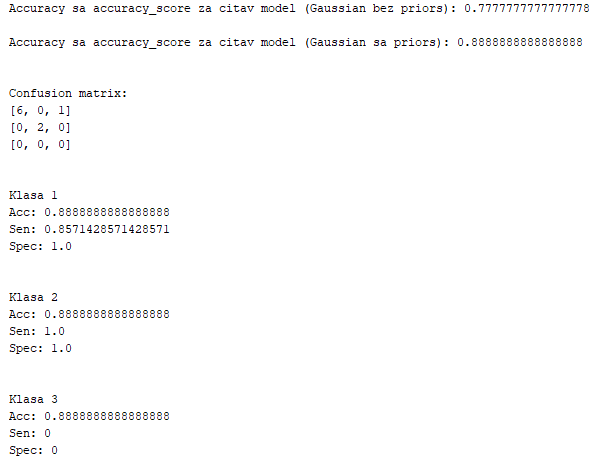
\includegraphics[scale=0.9]{slikaDrukcijaRaspodjela.png}
\caption{Rezultati pokretanja modela za prepoznavanje nakon ponovne raspodjele podataka}
	
\end{figure}

Vidljivo je da se tačnost modela povećala na oko \textbf{89\%}, te da su vrijednosti senzitivnosti i specifičnosti za klase 1 i 2 približno jednake 1, dok su za klasu 3 te vrijednosti opale na nulu. Ovo je posljedica \textit{overfitting}-a, odnosno zbog prevelikog treninga (nad 80\% podataka) dolazi do \textit{false positive} detekcija ćelija na slikama koje ih ne sadrže, iz kojeg razloga su performanse za treću klasu ovako niske.

\subsection{Izbacivanje \textit{outlier}-a slika}

Za bolju raspodjelu podataka u postojeće klase implementirana je funkcija \texttt{kMeansClustering} koja vrši raspodjelu podataka u \textit{cluster}-e u okviru iterativnog postupka, koji se sastoji iz sljedećih akcija:

\begin{enumerate}

\item Inicijalizacija centroida koristeći nasumične vrijednosti;
\item Dodjela svih podataka \textit{cluster}-ima na osnovu najmanje euklidske udaljenosti od centroida;
\item Provjera da li je uslov završavanja ispunjen (konvergencija podataka ili maksimalan broj iteracija).

\end{enumerate}

U skladu s postupkom, funkcija \texttt{kMeansClustering} prima sljedeće parametre:

\begin{enumerate}

\item \texttt{matrix}: podaci koje je potrebno dodijeliti \textit{cluster}-ima;
\item \texttt{noOfClasses}: broj \textit{cluster}-a;
\item \texttt{outlierPercentage}: ukoliko postotak broja podataka u određenom \textit{cluster}-u bude manji od ovog parametra, svi podaci koji pripadaju tom \textit{cluster}-u biti će obrisani, jer predstavljaju izolovani skup podataka udaljen od ostalih;
\item \texttt{maxNoOfIterations}: maksimalni broj iteracija nakon kojeg će se postupak \textit{clustering}-a završiti, ukoliko prethodno ne dođe do konvergencije podataka. 

\end{enumerate}

Za testni set podataka koji je prethodno korišten pri treniranju i testiranju izvršena su sljedeća testiranja vršenja \textit{clustering}-a:

\begin{table}[H]
\centering
\begin{tabular}{|l|l|l|l|l|}
\hline
\textbf{\texttt{noOfClasses}} 		& \textbf{\texttt{outlierPercentage}}   	& \textbf{ \texttt{maxNoOfIterations}} 		& \textbf{Rezultujući \textit{cluster}-i} 		\\ \hline
3            						& 0.1 								& 10              							& [14, 16, 13]            				   	\\ \hline
3            						& 0.1 								& 100              							& [15, 22, 33]          				   		\\ \hline
3            						& 0.1 								& 1000              							& [19, 21, 20]          				   		\\ \hline
3           						& 0.2 								& 1000             							& [19, 20, 21]          					 	\\ \hline
3           						& 0.5 								& 1000             							& [0, 0, 0]              					 	\\ \hline
\end{tabular}
\end{table}

\newpage

Iz navedenih rezultata vidljivo je da se s povećanjem broja iteracija dobiva veća pouzdanost \textit{clustering}-a, budući da početna konfiguracija centroida ovisi o nasumičnim vrijednostima. Iz tog razloga testiranja za veći broj klasa (kako bi se demonstriralo brisanje \textit{outlier}-a) biti će izvršeno koristeći vrijednost iteracija koja je veoma velika, da bi broj dodijeljenih elemenata u svim \textit{cluster}-ima bio pretežno identičan za sve različite veličine postotka za \textit{outlier}-e.

\begin{table}[H]
\centering
\begin{tabular}{|l|l|l|l|l|}
\hline
\textbf{\texttt{noOfClasses}} 		& \textbf{\texttt{outlierPercentage}}   	& \textbf{ \texttt{maxNoOfIterations}} 		& \textbf{Rezultujući \textit{cluster}-i} 		\\ \hline
4            						& 0.1 								& 1000              							& [14, 10, 20, 16]            				   	\\ \hline
4            						& 0.2 								& 1000              							& [19, 0, 21, 13]      				   		\\ \hline
4            						& 0.3 								& 1000              							& [0, 0, 20, 0]          				   		\\ \hline
6           						& 0.1 								& 1000             							& [0, 14, 14, 0, 16, 10]				 	\\ \hline
6           						& 0.2 								& 1000             							& [16, 14, 0, 0, 0, 0] 					 	\\ \hline
6           						& 0.3 								& 1000             							& [0, 0, 0, 0, 0, 0]    					 	\\ \hline
\end{tabular}
\end{table}

Iz navedenih rezultata vidljivo je da se s povećanjem postotka koji se koristi kako bi se odredilo da je određeni \textit{cluster} potrebno obrisati, kao posljedica povećanja klasa i sve manjeg broja podataka u pojedinačnim \textit{cluster}-ima, povećava i broj obrisanih \textit{cluster}-a, odnosno \textit{cluster}-a koji se proglašavaju \textit{outlier}-ima.\\
Nakon vršenja \textit{clustering}-a izvršeno je novo testiranje modela, te su postignute sljedeće performanse:

\begin{figure}[H]

\center
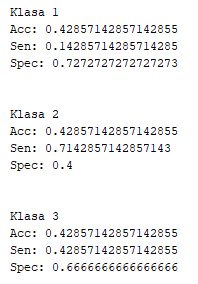
\includegraphics[scale=0.9]{slikaClustering.png}
\caption{Rezultati pokretanja modela za prepoznavanje nakon vršenja \textit{clustering}-a}
	
\end{figure}

Vidljivo je da je tačnost modela pala na čak \textbf{42.9 \%}, što je i očekivano, budući da je pri \textit{clustering}-u korištena metoda Euklidske distance, koja nije adekvatno mjerilo pripadnosti deskriptora određenim klasama.\\

\newpage

Treniranje modela urađeno je i bez vršenja dodjele klasa podacima nakon \textit{clustering}-a, pri čemu je postignuta tačnost modela od \textbf{86 \%} (koja je identična tačnosti modela bez vršenja \textit{clustering}-a) za sljedeće vrijednosti parametara:

\[\texttt{noOfClasses = 4 - 12, outlierPercentage = 0.05}\]

Za sve druge vrijednosti navedenih parametra postignute su gore performanse (npr. za broj klasa jednak 13 tačnost modela je oko 81 \%). Ovo je indikacija da se uklanjanjem određenog dijela podataka na ovaj način ne mogu postići bolje performanse od inicijalnih, budući da podaci ne samo da su ispravno grupisani, već uklanjanje jednog dijela njih za posljedicu ima nedovoljnu istreniranost modela kako bi testiranje bilo uspješno.

\begin{figure}[H]

\center
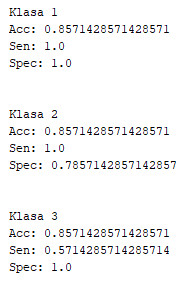
\includegraphics[scale=0.9]{slikaClustering2.png}
\caption{Rezultati pokretanja modela za prepoznavanje nakon vršenja \textit{clustering}-a bez dodjele klasa}
	
\end{figure}

\newpage

\subsection{Proširenje \textit{dataset}-a}

\textit{Dataset} je proširen sa ukupno \textbf{60 slika}, tako da je ukupan broj slika porastao sa 90 na 150, a broj slika po klasi sa 30 na 50 slika. Nakon vršenja novog izdvajanja i modifikacije ROI-a, izdvajanja deskriptora te treniranja i testiranja modela, postignuti su sljedeći rezultati:

\begin{figure}[H]

\center
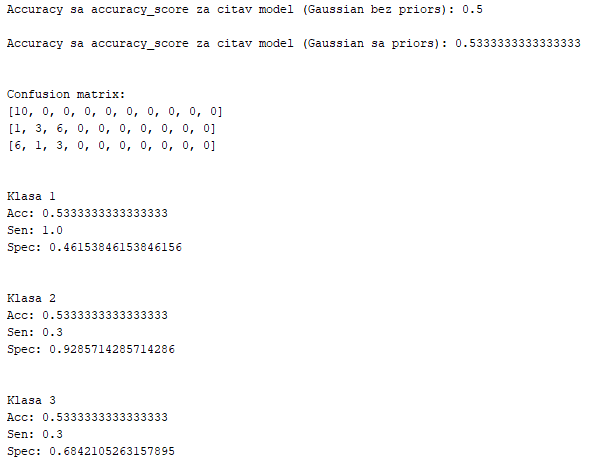
\includegraphics[scale=0.9]{slikaExtended.png}
\caption{Rezultati pokretanja modela za prepoznavanje nakon vršenja proširenja \textit{dataset}-a}
	
\end{figure}

Vidljivo je da je tačnost modela spala na oko \textbf{54\%}, što je dokaz da vršenje ovakvog proširenja \textit{dataset}-a ne samo da nije pozitivno utjecalo na moć detekcije, već je zbog prevelike količine informacije uzrokovalo pogoršanje modela za detekciju. Senzitivnost klase 1 ostala je maksimalna (1.0), dok su se senzitivnosti klasa 2 i 3 drastično smanjile, što dovodi do zaključka da je model previše istreniran za podatke iz klase 1, te da većinu podataka pogrešno dodjeljuje toj klasi, te da ga je potrebno dodatno trenirati na ostale dvije klase kako bi se njihova senzitivnost povećala.

\end{document}